\documentclass[12pt,a4paper]{article}

% ─── Page Layout ───────────────────────────────────────────────────────────────
\usepackage[a4paper, margin=0.8in, headheight=14pt]{geometry}

% ─── Fonts (XeLaTeX) ───────────────────────────────────────────────────────────
\usepackage{fontspec}
\usepackage{unicode-math}
\setmainfont{TeX Gyre Pagella}
\setmonofont[Scale=0.88]{TeX Gyre Cursor}
\setmathfont{Latin Modern Math}

% ─── Packages ──────────────────────────────────────────────────────────────────
\usepackage{xcolor}
\usepackage{colortbl}
\usepackage{titlesec}
\usepackage{enumitem}
\usepackage{tabularx}
\usepackage{booktabs}
\usepackage{array}
\usepackage{amsmath}
\usepackage{tikz}
\usetikzlibrary{shapes.geometric, arrows.meta, positioning, calc, fit, decorations.pathreplacing}
\usepackage{tcolorbox}
\tcbuselibrary{skins, breakable}
\usepackage{hyperref}
\usepackage{fancyhdr}
\usepackage{graphicx}
\usepackage{microtype}
\hyphenpenalty=10000
\exhyphenpenalty=10000
\sloppy
\usepackage{caption}
\usepackage{setspace}
\usepackage{multirow}
\usepackage{tocloft}

% ─── Q&A helper ────────────────────────────────────────────────────────────────
\newcommand{\Q}[1]{\textbf{#1}\par\noindent\ignorespaces}

% ─── Colour Palette ────────────────────────────────────────────────────────────
\definecolor{myred}{RGB}{196,30,58}
\definecolor{mydark}{RGB}{30,30,50}
\definecolor{mygreen}{RGB}{14,120,80}
\definecolor{myteal}{RGB}{0,130,140}
\definecolor{myamber}{RGB}{180,100,0}
\definecolor{mypurple}{RGB}{100,30,160}
\definecolor{mygray}{RGB}{246,247,249}
\definecolor{mgframe}{RGB}{180,185,200}
\definecolor{watermark}{RGB}{145,150,170}
\definecolor{hdrred}{RGB}{250,232,235}
\definecolor{hdrgreen}{RGB}{220,244,233}
\definecolor{hdrteal}{RGB}{220,242,244}
\definecolor{hdramber}{RGB}{253,242,215}
\definecolor{hdrpurple}{RGB}{238,228,255}
\definecolor{hdrgray}{RGB}{238,240,245}
\definecolor{rowalt}{RGB}{250,251,253}

% ─── Section Formatting ────────────────────────────────────────────────────────
\titleformat{\section}
  {\large\bfseries\color{myred}}{\thesection.}{0.5em}{}
  [\vspace{1pt}{\color{myred}\rule{\linewidth}{0.8pt}}]
\titleformat{\subsection}
  {\normalsize\bfseries\color{myteal}}{\thesubsection}{0.5em}{}
\titlespacing*{\section}{0pt}{18pt}{7pt}
\titlespacing*{\subsection}{0pt}{11pt}{4pt}

% ─── Paragraph ─────────────────────────────────────────────────────────────────
\setlength{\parindent}{0pt}
\setlength{\parskip}{4pt}

% ─── TOC Styling ───────────────────────────────────────────────────────────────
\renewcommand{\cfttoctitlefont}{\large\bfseries\color{myred}}
\renewcommand{\cftaftertoctitle}{\par\noindent{\color{myred}\rule{\linewidth}{0.8pt}}}
\setlength{\cftbeforetoctitleskip}{0pt}
\setlength{\cftaftertoctitleskip}{6pt}
\renewcommand{\cftsecfont}{\normalsize\bfseries\color{mydark}}
\renewcommand{\cftsecpagefont}{\normalsize\bfseries\color{mydark}}
\renewcommand{\cftsecleader}{\cftdotfill{\cftdotsep}}
\setlength{\cftbeforesecskip}{7pt}
\renewcommand{\cftsubsecfont}{\small\color{mydark}}
\renewcommand{\cftsubsecpagefont}{\small\color{mydark}}
\setlength{\cftbeforesubsecskip}{3pt}
\setlength{\cftsubsecindent}{1.4em}

% ─── Table helpers ─────────────────────────────────────────────────────────────
\renewcommand{\arraystretch}{1.45}
\setlength{\tabcolsep}{6pt}
\arrayrulecolor{mydark}
\newcolumntype{B}[1]{>{\small\bfseries\raggedright\arraybackslash}m{#1}}
\newcolumntype{Y}{>{\small\raggedright\arraybackslash}X}
\renewcommand{\tabularxcolumn}[1]{m{#1}}

% ─── Header / Footer ───────────────────────────────────────────────────────────
\pagestyle{fancy}
\fancyhf{}
\fancyhead[L]{\small\color{myred}\textbf{PE-EC801A}\;\color{mydark}--- Antennas and Propagation}
\fancyhead[R]{\small\color{myteal}\textbf{Module 7 Notes}}
\fancyfoot[C]{\small\color{mydark}\thepage}
\fancyfoot[R]{\small\color{watermark}\textit{\copyright\ Biraj}}
\renewcommand{\headrulewidth}{0.5pt}
\renewcommand{\footrulewidth}{0.3pt}

% ─── Hyperref ──────────────────────────────────────────────────────────────────
\hypersetup{
  colorlinks=true, linkcolor=myteal, urlcolor=myteal,
  pdfauthor={Biraj Sarkar},
  pdftitle={PE-EC801A --- Module 7 Notes}
}

% ─── tcolorbox styles ──────────────────────────────────────────────────────────
\tcbset{
  tikzbox/.style={
    colback=mygray, colframe=mgframe, boxrule=0.6pt, arc=4pt,
    left=8pt, right=8pt, top=6pt, bottom=6pt,
    colbacktitle=mgframe, coltitle=mydark,
    fonttitle=\small\bfseries
  },
  defbox/.style={
    colback=hdrgreen, colframe=mygreen, boxrule=0.8pt, arc=4pt,
    left=9pt, right=9pt, top=6pt, bottom=6pt,
    colbacktitle=mygreen, coltitle=white,
    fonttitle=\small\bfseries
  },
  formulabox/.style={
    colback=hdrteal, colframe=myteal, boxrule=0.8pt, arc=4pt,
    left=9pt, right=9pt, top=7pt, bottom=7pt,
    colbacktitle=myteal, coltitle=white,
    fonttitle=\small\bfseries
  },
  examplebox/.style={
    colback=hdramber, colframe=myamber, boxrule=0.8pt, arc=4pt,
    left=9pt, right=9pt, top=6pt, bottom=6pt,
    colbacktitle=myamber, coltitle=white,
    fonttitle=\small\bfseries
  },
  masonbox/.style={
    colback=hdrpurple, colframe=mypurple, boxrule=0.8pt, arc=4pt,
    left=9pt, right=9pt, top=6pt, bottom=6pt,
    colbacktitle=mypurple, coltitle=white,
    fonttitle=\small\bfseries
  },
  exambox/.style={
    colback=hdrpurple, colframe=mypurple, boxrule=1pt, arc=5pt,
    left=10pt, right=10pt, top=8pt, bottom=8pt,
    colbacktitle=mypurple, coltitle=white,
    fonttitle=\bfseries,
    breakable, title after break={\textbf{Frequently Asked / Viva Questions (contd.)}}}
}
\tcbset{breakable}

% ─── TikZ styles ───────────────────────────────────────────────────────────────
\tikzset{
  block/.style={rectangle, draw=myteal, fill=hdrteal,
    text width=2.4cm, align=center, minimum height=0.95cm,
    font=\small, rounded corners=3pt, line width=0.7pt},
  redblock/.style={rectangle, draw=myred, fill=hdrred,
    text width=2.4cm, align=center, minimum height=0.95cm,
    font=\small, rounded corners=3pt, line width=0.7pt},
  netnode/.style={rectangle, draw=myteal, fill=hdrteal,
    text width=1.5cm, align=center, minimum height=0.8cm,
    font=\small, rounded corners=3pt, line width=0.7pt},
  sumjunc/.style={circle, draw=myamber, fill=hdramber,
    minimum size=0.62cm, font=\small, line width=0.8pt},
  snode/.style={circle, draw=mypurple, fill=hdrpurple,
    minimum size=0.55cm, font=\footnotesize, line width=0.7pt},
  arrow/.style={-Stealth, thick, color=mydark},
  redarrow/.style={-Stealth, thick, color=myred},
  line/.style={thick, color=mydark}
}

% ═══════════════════════════════════════════════════════════════════════════════
\begin{document}
% ═══════════════════════════════════════════════════════════════════════════════

\begin{center}
  {\LARGE\bfseries\color{myred} PE-EC801A --- Antennas and Propagation}\\[5pt]
  {\normalsize\color{mydark} Semester VIII \quad$\bullet$\quad 3L:0T:0P \quad$\bullet$\quad 3 Credits}\\[3pt]
  {\normalsize\color{myteal}\textbf{Module 7 Exam Notes}}\\[3pt]
  {\small\color{mydark} CGEC \;$|$\; B.Tech ECE (2023--27) \;$|$\; \textit{Biraj Sarkar}}
\end{center}
\vspace{2pt}
\noindent{\color{myred}\rule{\linewidth}{1.5pt}}
\vspace{2pt}

\hypersetup{linkcolor=mydark}
\tableofcontents
\hypersetup{linkcolor=myteal}
\newpage

% ===============================================================================
\section{Basic Concepts of Smart Antennas}
% ===============================================================================

\begin{tcolorbox}[defbox, title={\textbf{Definition of Smart Antennas}}]
A \textbf{smart antenna} (or adaptive array) system combines an antenna array with digital signal processing (DSP) algorithms to automatically optimize its radiation pattern in response to the signal environment, steering beams toward desired users and placing nulls toward interferers.
\end{tcolorbox}

\subsection{Smart Antenna Architecture}
A typical smart antenna receiver consists of an antenna array, an RF downconverter, analog-to-digital converters (ADCs), and a digital signal processor (DSP).

\begin{tcolorbox}[tikzbox, title={Smart Antenna Receiver Block Diagram}]
\centering
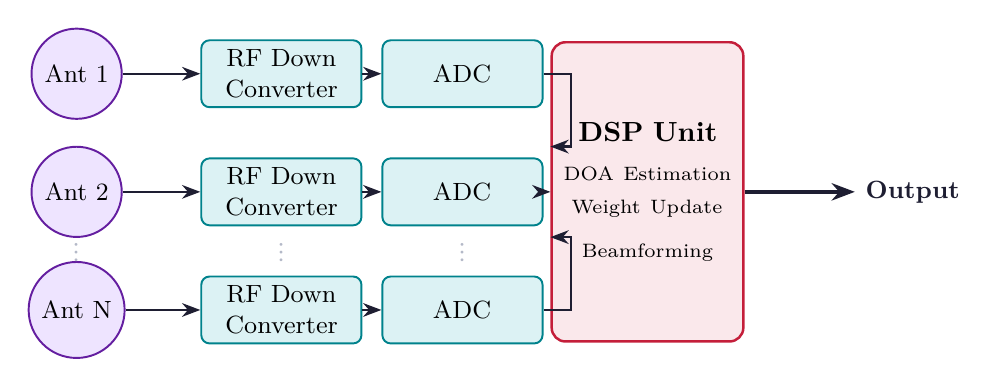
\begin{tikzpicture}[
  sblock/.style={rectangle, draw=myteal, fill=hdrteal, text width=1.8cm,
    align=center, minimum height=0.85cm, font=\small,
    rounded corners=3pt, line width=0.7pt},
  ablock/.style={circle, draw=mypurple, fill=hdrpurple,
    minimum size=0.72cm, font=\small, line width=0.7pt}]

  % ── Row y-coordinates: evenly spaced ─────────────────────────────────────
  % Row 1 (Ant 1) at y=1.5, Row 2 (Ant 2) at y=0, Row N at y=-1.5
  % Dot row midway between rows 2 and N at y=-0.75

  % ── Column x-coordinates ──────────────────────────────────────────────────
  % Ant: x=0, RF: x=2.4, ADC: x=4.65, DSP: x=7.0

  % ── Antenna column ────────────────────────────────────────────────────────
  \node[ablock] (a1) at (0,  1.5) {Ant 1};
  \node[ablock] (a2) at (0,  0.0) {Ant 2};
  \node[ablock] (aN) at (0, -1.5) {Ant N};

  % ── RF Downconverter column ───────────────────────────────────────────────
  \node[sblock] (rf1) at (2.6,  1.5) {RF Down\\Converter};
  \node[sblock] (rf2) at (2.6,  0.0) {RF Down\\Converter};
  \node[sblock] (rfN) at (2.6, -1.5) {RF Down\\Converter};

  % ── ADC column ────────────────────────────────────────────────────────────
  \node[sblock] (adc1) at (4.9,  1.5) {ADC};
  \node[sblock] (adc2) at (4.9,  0.0) {ADC};
  \node[sblock] (adcN) at (4.9, -1.5) {ADC};

  % ── DSP Unit — centred at y=0, height spans all 3 rows ────────────────────
  \node[draw=myred, fill=hdrred, line width=0.9pt, rounded corners=5pt,
        minimum height=3.8cm, text width=2.2cm, align=center]
       (dsp) at (7.25, 0)
       {\textbf{DSP Unit}\\[6pt]
        \scriptsize DOA Estimation\\[4pt]
        \scriptsize Weight Update\\[4pt]
        \scriptsize Beamforming};

  % ── Dot rows — centred in the gap between row 2 and row N ─────────────────
  \node[font=\normalsize, color=mgframe] at (0,   -0.77) {$\vdots$};
  \node[font=\normalsize, color=mgframe] at (2.6, -0.77) {$\vdots$};
  \node[font=\normalsize, color=mgframe] at (4.9, -0.77) {$\vdots$};

  % ── Connections — row 1 ───────────────────────────────────────────────────
  \draw[arrow] (a1)   -- (rf1);
  \draw[arrow] (rf1)  -- (adc1);
  \draw[arrow] (adc1.east) -- ++(0.35,0) |- (dsp.155);

  % ── Connections — row 2 ───────────────────────────────────────────────────
  \draw[arrow] (a2)   -- (rf2);
  \draw[arrow] (rf2)  -- (adc2);
  \draw[arrow] (adc2.east) -- (dsp.west);

  % ── Connections — row N ───────────────────────────────────────────────────
  \draw[arrow] (aN)   -- (rfN);
  \draw[arrow] (rfN)  -- (adcN);
  \draw[arrow] (adcN.east) -- ++(0.35,0) |- (dsp.205);

  % ── Output ────────────────────────────────────────────────────────────────
  \draw[arrow, line width=1.2pt] (dsp.east) -- ++(1.4,0)
    node[right, font=\small\bfseries\color{mydark}] {Output};

\end{tikzpicture}
\end{tcolorbox}

\subsection{Beamforming Basics}
\begin{itemize}[leftmargin=*, itemsep=3pt]
  \item \textbf{Phased Array / Fixed-Weight Beamforming:} The weights (amplitudes and phases) are predefined or adjusted using analog phase shifters to steer the main beam in a specific fixed direction.
  \item \textbf{Adaptive Beamforming:} The weights are dynamically computed in real-time by a DSP processor using feedback algorithms to optimize the Signal-to-Interference-plus-Noise Ratio (SINR).
  \item \textbf{Algorithms:} Common adaptive weight-updating algorithms include:
    \begin{itemize}[leftmargin=*, itemsep=1pt]
      \item \textbf{LMS (Least Mean Squares):} Low complexity, gradient descent.
      \item \textbf{RLS (Recursive Least Squares):} Fast convergence, high complexity.
      \item \textbf{MUSIC / ESPRIT:} High-resolution algorithms used to find the Direction of Arrival (DOA) of incoming signals.
    \end{itemize}
\end{itemize}

\subsection{Weight Vector Formulation}
Let the $N$-element array receive a signal. The received signal vector is:
\[
\mathbf{x}(t) = [x_1(t),\ x_2(t),\ \dots,\ x_N(t)]^T
\]
The array output is a linear combination of the received signals weighted by a complex weight vector $\mathbf{w} = [w_1, w_2, \dots, w_N]^T$:
\[
y(t) = \mathbf{w}^H \mathbf{x}(t) = \sum_{n=1}^{N} w_n^* x_n(t)
\]
where $(\cdot)^H$ denotes the Hermitian (conjugate transpose). The weights control both the amplitude and phase applied to each antenna element output.

\textbf{Fixed-weight (Conventional) Beamformer:} For steering toward direction $\theta_0$, the optimal weights are the \textbf{steering vector} $\mathbf{a}(\theta_0)$:
\[
\mathbf{w} = \mathbf{a}(\theta_0) = [1,\ e^{j\psi},\ e^{j2\psi},\ \dots,\ e^{j(N-1)\psi}]^T, \quad \psi = kd\cos\theta_0
\]
This applies a phase ramp across the array to align and coherently add the signals from direction $\theta_0$.

\subsection{LMS Adaptive Algorithm}
The \textbf{Least Mean Squares (LMS)} algorithm updates the weight vector iteratively to minimize the mean square error between the array output $y(k)$ and a reference signal $d(k)$ (desired signal):

\begin{tcolorbox}[formulabox, title={\textbf{LMS Weight Update Rule}}]
\[
e(k) = d(k) - \mathbf{w}^H(k)\,\mathbf{x}(k) \quad \text{(error signal)}
\]
\[
\mathbf{w}(k+1) = \mathbf{w}(k) + 2\mu\, \mathbf{x}(k)\, e^*(k) \quad \text{(weight update)}
\]
where $\mu$ is the step-size parameter ($0 < \mu < \frac{1}{N \cdot P_{in}}$, $P_{in}$ = input power).
\end{tcolorbox}

\begin{itemize}[leftmargin=*, itemsep=2pt]
  \item \textbf{Small $\mu$:} Slow convergence, low misadjustment (stable, accurate steady state).
  \item \textbf{Large $\mu$:} Fast convergence, high misadjustment (may diverge if too large).
  \item The LMS algorithm steers the main beam toward the desired user while automatically placing nulls in the directions of interferers — no explicit knowledge of interferer locations is needed.
\end{itemize}

\begin{tcolorbox}[tikzbox, title={Switched-Beam vs. Adaptive Array Patterns}]
\centering
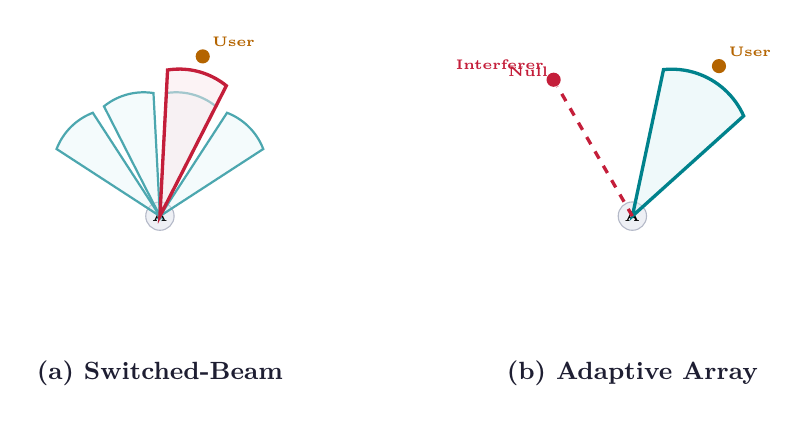
\begin{tikzpicture}[scale=1.0]
  % ── (a) Switched-Beam ──────────────────────────────────────────────────────
  \begin{scope}[xshift=-3.0cm]
    % Array element at centre
    \fill[hdrgray, draw=mgframe] (0,0) circle (0.18);
    \node[font=\tiny\bfseries] at (0,0) {A};

    % Four fixed beams as filled wedges (using proper polar coords)
    % Beam angles from vertical: 45, 75, 105, 135 deg (measured from positive x-axis)
    \foreach \ang/\hw in {45/12, 75/12, 105/12, 135/12} {
      \draw[color=myteal!70, fill=hdrteal, fill opacity=0.30, thick,
            domain={-\hw}:{\hw}, samples=20, variable=\r]
        plot ({1.6*cos(\r)*cos(\ang + \r)}, {1.6*cos(\r)*sin(\ang + \r)}) -- (0,0) -- cycle;
    }
    % Active (selected) beam highlighted in red — beam at 75 deg
    \draw[color=myred, fill=hdrred, fill opacity=0.5, very thick,
          domain=-12:12, samples=20, variable=\r]
      plot ({1.9*cos(\r)*cos(75 + \r)}, {1.9*cos(\r)*sin(75 + \r)}) -- (0,0) -- cycle;

    % User dot
    \fill[myamber] ({2.1*cos(75)},{2.1*sin(75)}) circle (0.09)
      node[above right, font=\tiny\bfseries\color{myamber}] {User};

    \node[font=\small\bfseries\color{mydark}] at (0,-2.0) {(a) Switched-Beam};
  \end{scope}

  % ── (b) Adaptive Array ─────────────────────────────────────────────────────
  \begin{scope}[xshift=3.0cm]
    % Array element
    \fill[hdrgray, draw=mgframe] (0,0) circle (0.18);
    \node[font=\tiny\bfseries] at (0,0) {A};

    % Steered beam toward user at 60 deg (narrow)
    \draw[color=myteal, fill=hdrteal, fill opacity=0.45, very thick,
          domain=-18:18, samples=25, variable=\r]
      plot ({2.0*cos(\r)*cos(60 + \r)}, {2.0*cos(\r)*sin(60 + \r)}) -- (0,0) -- cycle;

    % Null line toward interferer at 120 deg
    \draw[very thick, color=myred, dashed] (0,0) -- ({1.9*cos(120)},{1.9*sin(120)});
    \node[above left, font=\tiny\bfseries\color{myred}] at ({1.9*cos(120)},{1.9*sin(120)}) {Null};

    % User and interferer dots
    \fill[myamber] ({2.2*cos(60)},{2.2*sin(60)}) circle (0.09)
      node[above right, font=\tiny\bfseries\color{myamber}] {User};
    \fill[myred] ({2.0*cos(120)},{2.0*sin(120)}) circle (0.09)
      node[above left, font=\tiny\bfseries\color{myred}] {Interferer};

    \node[font=\small\bfseries\color{mydark}] at (0,-2.0) {(b) Adaptive Array};
  \end{scope}
\end{tikzpicture}
\end{tcolorbox}

% ===============================================================================
\section{Radio Wave Propagation Modes}
% ===============================================================================

Radio waves propagate from transmitter to receiver via three primary modes depending on their frequency.

\begin{tcolorbox}[tikzbox, title={Radio Wave Propagation Modes}]
\centering
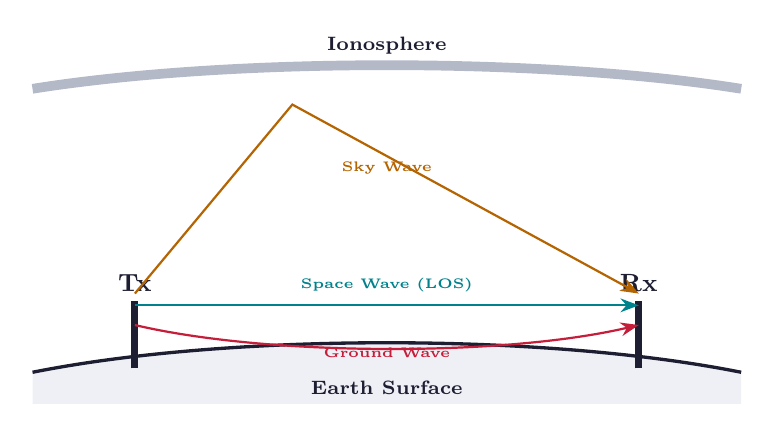
\begin{tikzpicture}[scale=1.0]
  % ── Earth surface (gentle arc, bounded) ────────────────────────────────────
  \fill[hdrgray] (-4.5,-1.4) .. controls (-2,-0.9) and (2,-0.9) .. (4.5,-1.4) --
                 (4.5,-1.8) -- (-4.5,-1.8) -- cycle;
  \draw[very thick, color=mydark] (-4.5,-1.4) .. controls (-2,-0.9) and (2,-0.9) .. (4.5,-1.4);
  \node[font=\scriptsize\bfseries\color{mydark}] at (0,-1.6) {Earth Surface};

  % ── Ionosphere (arc at top, bounded) ───────────────────────────────────────
  \draw[line width=3.5pt, color=mgframe]
    (-4.5, 2.2) .. controls (-2, 2.6) and (2, 2.6) .. (4.5, 2.2);
  \node[font=\scriptsize\bfseries\color{mydark}] at (0, 2.75) {Ionosphere};

  % ── Tx and Rx towers ───────────────────────────────────────────────────────
  \draw[line width=2.5pt, color=mydark] (-3.2,-1.35) -- (-3.2,-0.5);
  \node[above, font=\small\bfseries\color{mydark}] at (-3.2,-0.5) {Tx};

  \draw[line width=2.5pt, color=mydark] (3.2,-1.35) -- (3.2,-0.5);
  \node[above, font=\small\bfseries\color{mydark}] at (3.2,-0.5) {Rx};

  % ── 1. Ground Wave ─────────────────────────────────────────────────────────
  \draw[thick, color=myred, -Stealth]
    (-3.2,-0.8) .. controls (-1.5,-1.2) and (1.5,-1.2) .. (3.2,-0.8);
  \node[font=\tiny\bfseries\color{myred}] at (0,-1.15) {Ground Wave};

  % ── 2. Space Wave (LOS) ────────────────────────────────────────────────────
  \draw[thick, color=myteal, -Stealth] (-3.2,-0.55) -- (3.2,-0.55);
  \node[above, font=\tiny\bfseries\color{myteal}] at (0,-0.5) {Space Wave (LOS)};

  % ── 3. Sky Wave ────────────────────────────────────────────────────────────
  \draw[thick, color=myamber, -Stealth]
    (-3.2,-0.4) -- (-1.2, 2.0) -- (3.2,-0.4);
  \node[font=\tiny\bfseries\color{myamber}] at (0, 1.2) {Sky Wave};
\end{tikzpicture}
\end{tcolorbox}

\subsection{Ground Wave (Surface Wave) Propagation}
Ground waves travel along the surface of the Earth, guided by the boundary between the atmosphere and the ground.
\begin{itemize}[leftmargin=*, itemsep=2pt]
  \item \textbf{Frequency Range:} Very Low Frequency (VLF) to Medium Frequency (MF) ($< 2\,\text{MHz}$).
  \item \textbf{Mechanism:} The wave induces currents in the ground, causing attenuation. Attenuation increases rapidly with frequency, limiting this mode to low frequencies.
  \item \textbf{Application:} AM radio broadcasting, maritime communications.
\end{itemize}

\subsection{Space Wave (Line-of-Sight) Propagation}
Space waves travel through the troposphere directly from transmitter to receiver, or via ground reflection.
\begin{itemize}[leftmargin=*, itemsep=2pt]
  \item \textbf{Frequency Range:} Very High Frequency (VHF) and above ($> 30\,\text{MHz}$).
  \item \textbf{Radio Horizon ($d$):} The maximum line-of-sight distance is limited by the curvature of the Earth. Accounting for atmospheric refraction (effective Earth radius factor $k = 4/3$):
  \[
  d \approx \sqrt{17 h_t} + \sqrt{17 h_r} \approx 4.12 \left( \sqrt{h_t} + \sqrt{h_r} \right) \,\text{km}
  \]
  where $h_t$ and $h_r$ are the heights of the transmitting and receiving towers in meters.
  \item \textbf{Other modes:} Tropospheric scatter, duct propagation.
\end{itemize}

\subsection{Sky Wave Propagation}
Sky waves travel upward and are reflected (refracted) back to Earth by the ionosphere.
\begin{itemize}[leftmargin=*, itemsep=2pt]
  \item \textbf{Frequency Range:} High Frequency (HF) ($3$–$30\,\text{MHz}$).
  \item \textbf{Ionospheric Layers:} Formed by solar UV/X-ray ionization.
\end{itemize}

\par\noindent
\textbf{Ionosphere Layers Properties:}\par\noindent
{\renewcommand{\arraystretch}{1.45}%
\begin{tabularx}{\linewidth}{|B{1.5cm}|B{2.2cm}|Y|Y|}
\hline
\textbf{Layer} & \textbf{Altitude} & \textbf{Day Behavior} & \textbf{Night Behavior} \\
\hline
D Layer & $50$–$90\,\text{km}$ & Absorbs HF; reflects VLF/LF. & Disappears (recombines). \\
\hline
E Layer & $90$–$140\,\text{km}$ & Partially reflects HF. & Weakens significantly. \\
\hline
F1 Layer & $140$–$250\,\text{km}$ & Merges with F2 at night. & Disappears. \\
\hline
F2 Layer & $250$–$400\,\text{km}$ & Highest electron density; primary sky wave reflector. & Merges into a single F layer. \\
\hline
\end{tabularx}}

% ===============================================================================
\section{Ionospheric Parameters}
% ===============================================================================

The ionosphere acts as a refracting medium. Its refractive index $n$ is:
\[
n = \sqrt{1 - \frac{81 N}{f^2}}
\]
where $N$ is the electron density (electrons/$\text{m}^3$) and $f$ is the wave frequency (Hz).

\textbf{Physical Interpretation:} When a sky wave enters the ionosphere at an oblique angle, successive layers of increasing electron density bend the wave progressively away from vertical (like Snell's law in optics). Eventually, at the height where $n = \cos\theta_i$, the wave is totally reflected and returns to Earth. If the frequency is too high, $n$ never equals $\cos\theta_i$ and the wave escapes into space.

\subsection{Virtual Height}
The \textbf{virtual height} ($h_{virt}$) is the apparent height from which a short pulse of radio energy appears to be reflected, assuming the wave traveled at the speed of light in free space for the entire round trip. It is always greater than the actual reflection height because the wave slows down as electron density increases.
\[
h_{virt} = \frac{c \cdot \Delta t}{2}
\]
where $\Delta t$ is the round-trip time for a vertically launched pulse.

\subsection{Lowest Usable Frequency (LUF)}
The \textbf{LUF} is the lowest frequency at which sky-wave communication is possible over a given path. Below the LUF, the D-layer absorption becomes so severe that the signal is absorbed before reaching the receiver. The LUF depends on:
\begin{itemize}[leftmargin=*, itemsep=2pt]
  \item Solar activity (higher absorption during daytime and solar maxima).
  \item Path length and required signal level.
  \item Transmitter power (higher power lowers the effective LUF).
\end{itemize}
The \textbf{Optimum Working Frequency (OWF)} is typically chosen as $85\%$ of the MUF to provide a safety margin against day-to-day variability:
\[
f_{OWF} \approx 0.85 \times f_{MUF}
\]

\begin{tcolorbox}[formulabox, title={\textbf{Key Sky-Wave Design Parameters}}]
\begin{enumerate}[leftmargin=*, label=\textbf{\arabic*.}, itemsep=3pt, topsep=1pt]
  \item \textbf{Critical Frequency ($f_c$):} The highest frequency that is reflected back to Earth when launched vertically ($90^\circ$ elevation):
  \[
  f_c = 9\sqrt{N_{max}}
  \]
  where $N_{max}$ is the maximum electron density in the reflecting layer (electrons/m$^3$).
  \item \textbf{Maximum Usable Frequency (MUF):} The highest frequency reflected back to Earth when launched at an oblique angle of incidence $\theta_i$ (measured from vertical):
  \[
  f_{MUF} = f_c \sec\theta_i = \frac{f_c}{\cos\theta_i} \quad (\text{Secant Law})
  \]
  For a flat Earth approximation with path length $D$ and reflection height $h$:
  \[
  \sec\theta_i = \sqrt{1 + \left(\frac{D}{2h}\right)^{\!2}}
  \]
  \item \textbf{Skip Distance ($D_{skip}$):} The minimum distance from the transmitter where a sky wave of frequency $f$ ($f > f_c$) returns to Earth. Within this distance, no sky-wave signal is received — this region is called the \textbf{skip zone}:
  \[
  D_{skip} = 2 h_{virt} \sqrt{\left(\frac{f_{MUF}}{f_c}\right)^{\!2} - 1}
  \]
  \item \textbf{Optimum Working Frequency (OWF):}
  \[
  f_{OWF} \approx 0.85 \times f_{MUF}
  \]
\end{enumerate}
\end{tcolorbox}

\subsection{Skip Zone and Dead Zone}
\begin{itemize}[leftmargin=*, itemsep=3pt]
  \item \textbf{Skip Zone (Dead Zone):} The annular region around the transmitter where neither the ground wave (which has died out) nor the sky wave (which overshoots) can be received. For a sky wave of frequency $f$, the inner edge of the skip zone is at the skip distance $D_{skip}$.
  \item \textbf{Effect of Frequency:} As frequency increases toward the MUF, the skip distance increases. As frequency decreases toward $f_c$, the skip distance decreases to zero (the wave returns almost vertically).
  \item \textbf{Multiple Hops:} Sky waves can undergo successive reflections between the ionosphere and the Earth's surface, allowing communication over very long distances ($> 10{,}000\,\text{km}$).
\end{itemize}

% ===============================================================================
% MANDATORY QUICK REVISION PAGE
% ===============================================================================
\newpage
\begin{center}
  {\large\bfseries\color{myred} Quick Revision --- Module 7}\\[3pt]
  {\small\color{mydark} Smart Antennas and Propagation $|$ PE-EC801A}
\end{center}
\noindent{\color{myred}\rule{\linewidth}{1.2pt}}
\vspace{4pt}

\begin{tcolorbox}[formulabox, title={\textbf{Key Formulas and Metrics at a Glance}}]
\renewcommand{\arraystretch}{1.35}
\begin{tabularx}{\linewidth}{B{5.2cm} X}
Radio Horizon Distance ($d$) & $d \approx 4.12 (\sqrt{h_t} + \sqrt{h_r})$ \quad (in km, $h$ in meters) \\[4pt]
Ionospheric Refractive Index ($n$) & $n = \sqrt{1 - \frac{81 N}{f^2}}$ \\[4pt]
Critical Frequency ($f_c$) & $f_c = 9\sqrt{N_{max}}$ \quad (vertical incidence) \\[4pt]
Oblique Secant Law (MUF) & $f_{MUF} = f_c \sec\theta_i$ \\[4pt]
Skip Distance ($D_{skip}$) & $D_{skip} = 2 h \sqrt{(f_{MUF}/f_c)^2 - 1}$ \\[4pt]
Smart Weight Vector ($\vec{w}$) & $\vec{y}(t) = \vec{w}^H \vec{x}(t)$ \quad (combining array outputs) \\
\end{tabularx}
\end{tcolorbox}

\begin{tcolorbox}[defbox, title={\textbf{One-Line Definitions}}]
\begin{itemize}[leftmargin=*, itemsep=2pt, topsep=0pt]
  \item \textbf{DOA Estimation:} Direction of Arrival; calculating the angle from which a signal hits the antenna array.
  \item \textbf{Adaptive Beamforming:} Real-time DSP weight adjustment to maximize wanted signals and null out noise/interference.
  \item \textbf{Ground Wave:} A low-frequency electromagnetic wave that travels guided by the curvature and conductivity of the Earth.
  \item \textbf{Skip Distance:} The minimum distance from a transmitter where sky wave signals return to the Earth's surface.
  \item \textbf{Critical Frequency:} The limit frequency below which waves return to Earth at vertical incidence, and above which they escape to space.
  \item \textbf{Duct Propagation:} The trapping of VHF/UHF waves in a tropospheric layer due to temperature inversions, allowing long-range propagation.
\end{itemize}
\end{tcolorbox}

\begin{tcolorbox}[exambox, title={\textbf{Frequently Asked / Viva Questions}}]
\begin{enumerate}[topsep=0pt, label=\textbf{Q\arabic*.}, itemsep=5pt]
  \item \Q{What are the benefits of using smart antennas in wireless networks?}
    Smart antennas increase system capacity (via Space Division Multiple Access - SDMA), extend coverage range (via directive beam gain), reduce co-channel interference (by steering nulls toward interferers), and mitigate multipath fading.
  \item \Q{Compare switched-beam and adaptive array smart antennas.}
    Switched-beam systems select from a set of predefined, fixed beams. Adaptive arrays continuously track the user's location and steer the beam and nulls dynamically using DSP algorithms, offering higher performance but at a higher cost.
  \item \Q{Explain the physical mechanism of ground wave propagation. Why is it limited to low frequencies?}
    As ground waves travel, they induce currents in the Earth's surface. Since the Earth acts as a lossy dielectric, it dissipates power. Ground attenuation increases rapidly with frequency, limiting this mode to frequencies below $2\,\text{MHz}$.
  \item \Q{Define critical frequency, MUF, and skip zone.}
    \begin{itemize}[leftmargin=*, itemsep=1pt, topsep=2pt]
      \item \textbf{Critical Frequency ($f_c$):} The maximum frequency reflected at vertical incidence.
      \item \textbf{MUF:} The maximum frequency reflected at oblique incidence ($f_{MUF} = f_c \sec\theta_i$).
      \item \textbf{Skip Zone:} The region between the limit of ground-wave coverage and the point where the first sky-wave returns to Earth. No signal is received in this zone.
    \end{itemize}
  \item \Q{Why does the D-layer of the ionosphere disappear at night?}
    The D-layer is the lowest layer ($50$–$90\,\text{km}$) where atmospheric density is high. It is ionized during the day by solar radiation. At night, without solar rays, free electrons recombine rapidly with ions due to the high collision rate, causing the layer to disappear.
  \item \Q{State the formula for the line-of-sight range of space waves. How does the earth's atmosphere affect it?}
    $d \approx 4.12 (\sqrt{h_t} + \sqrt{h_r})$ km. The atmosphere has a refractive index that decreases with height, which bends waves slightly downward, extending the radio horizon about $15\%$ beyond the geometric optical horizon. This is modeled using an effective Earth radius factor $k = 4/3$.
\end{enumerate}
\end{tcolorbox}

\begin{tcolorbox}[tikzbox, title={Comparison of Wave Propagation Modes}]
\centering
\renewcommand{\arraystretch}{1.55}
{\renewcommand{\arraystretch}{1.55}%
\begin{tabularx}{\linewidth}{|B{3.2cm}|Y|Y|Y|}
\hline
\multicolumn{1}{|>{\centering\arraybackslash}m{3.2cm}|}{\textbf{Parameter}} &
\multicolumn{1}{>{\centering\arraybackslash}Y|}{\textbf{Ground Wave}} &
\multicolumn{1}{>{\centering\arraybackslash}Y|}{\textbf{Space Wave}} &
\multicolumn{1}{>{\centering\arraybackslash}Y|}{\textbf{Sky Wave}} \\
\hline
Frequency Range & $< 2\,\text{MHz}$ (LF/MF) & $> 30\,\text{MHz}$ (VHF/UHF/SHF) & $3$–$30\,\text{MHz}$ (HF) \\
\hline
Propagation Path & Curves along Earth's surface & Direct line-of-sight path & Ionospheric reflection/refraction \\
\hline
Primary Limitation & High ground attenuation at higher frequencies & Earth curvature blockage (radio horizon) & Solar ionization variations (day/night/seasonal) \\
\hline
Typical Applications & AM radio, maritime navigation & FM, TV, cellular, satellite & Long-range amateur radio, SW broadcasting \\
\hline
\end{tabularx}}
\end{tcolorbox}

\end{document}
